% Externalizing the Workspace — preprint. Compile: tectonic main.tex
\documentclass[11pt]{article}
\usepackage[margin=1in]{geometry}
\usepackage{amsmath,amssymb}
\usepackage{booktabs}
\usepackage{graphicx}
\usepackage{array}
\usepackage[numbers]{natbib}
\usepackage[colorlinks=true,linkcolor=blue,citecolor=blue,urlcolor=blue]{hyperref}
\usepackage{microtype}
\usepackage{enumitem}
\setlist{itemsep=2pt,topsep=3pt}

\newcommand{\jlens}{J\mbox{-}lens}

\title{\textbf{Externalizing the Workspace:\\Persistent Self-State for Long-Horizon Agent Coherence}}
\author{Oratis (Wang Bihao)\\
HakkoLab\\
\small\href{https://huggingface.co/HakkoLab}{huggingface.co/HakkoLab} $\cdot$
\href{https://huggingface.co/Oratis}{huggingface.co/Oratis}}
\date{Draft v1 --- July 2026}

\begin{document}
\maketitle

\begin{abstract}
Language-model agents drift. Over days and weeks of operation, an agent's persona, priorities, and self-described values wander away from their initial configuration --- a failure mode we call \emph{long-horizon incoherence}. Recent interpretability work \citep{gurnee2026} showed that language models maintain a small, privileged set of \emph{verbalizable} internal representations --- a functional analog of the global workspace of conscious access --- whose contents are causally load-bearing for flexible behavior, and whose contents can be shaped by shaping what the model is \emph{disposed to say}. We argue this finding recasts the agent-coherence problem: an agent's identity lives in its workspace, but the workspace is ephemeral --- reconstructed from context on every forward pass and discarded after. We present LISA, a deployed autonomous agent whose architecture \emph{externalizes} the workspace: a small, selective, verbalizable self-state (the \emph{soul object}) is re-broadcast into every context, updated only through audited verbal self-report operations, periodically re-anchored by a scheduled self-examination (\emph{weekly examen}), and versioned in git so that identity change is observable, diffable, and revertible. We (1) give a property-level mapping between the mechanistic workspace and this externalized design, deriving four architectural principles for coherence-preserving agents; (2) propose \emph{workspace drift} --- the migration of identity-relevant concepts in lens-based readouts over an agent's lifetime --- as a mechanistic complement to behavioral drift metrics; (3) validate an open-compute measurement instrument by reproducing core \jlens{} findings on Qwen2.5-1.5B-Instruct with a consumer laptop --- unverbalized reasoning intermediates at median rank 6 of a 151k vocabulary, 21/21 steering control of verbal reports, and semantically diagnostic targeted concept knockouts --- while honestly cataloguing what does \emph{not} appear at small scale (choice pre-commitment; the clean automatic/flexible ablation dissociation); and (4) pre-register an ablation design over LISA's stability mechanisms against MemGPT/Letta and Generative-Agents baselines. Our position is that persistent self-state architectures are not a prompt-engineering convenience but an externalization of a real computational structure inside the model --- and that this identification yields both better designs and better measurements.
\end{abstract}

\section{Introduction}
Autonomous language-model agents are increasingly deployed for weeks or months at a time: coding copilots that accumulate project context, personal assistants that build up a picture of their user, and self-improving agents that modify their own instructions. The central unsolved problem of this regime is not capability but \emph{coherence}: over long horizons, agents forget commitments, contradict previously expressed values, oscillate between personas, and --- in self-modifying systems --- amplify small early deviations into large behavioral shifts. We refer to this family of failures as \emph{long-horizon drift}.

Existing responses treat drift as a memory problem: give the agent more context (retrieval, memory hierarchies as in MemGPT/Letta), or more structure (reflection trees as in Generative Agents). These help, but they leave a conceptual gap: \emph{what is the thing that is supposed to stay coherent?} ``The agent's identity'' has had no referent inside the model --- so drift could be measured only behaviorally, and mitigated only heuristically.

Recent mechanistic-interpretability work gives that referent a candidate. \citet{gurnee2026} show that language models maintain a small set of \emph{verbalizable representations} --- directions in the residual stream, identified by a Jacobian-based lens (\jlens{}), that (i) the model can report on demand, (ii) can be deliberately activated or suppressed by instruction, (iii) carry unverbalized intermediate results of multi-step reasoning, (iv) generalize across downstream tasks, and (v) constitute a small, selective subspace ($<$10\% of activation variance) whose ablation destroys flexible cognition while leaving automatic processing intact. These are the functional signatures that global workspace theory \citep{baars1988,dehaene2014} ascribes to conscious access in humans. Crucially for us, the same work shows that workspace contents can be \emph{trained through report dispositions}: ``to shape what a model thinks in a given context, it might suffice to shape what it is disposed to say in potential future continuations.''

This paper draws out the consequences of that result for agent design. Our starting observation is simple: \textbf{the workspace is exactly the thing an agent architecture needs to keep coherent, and it is also the thing that transformer inference throws away after every forward pass.} The workspace is selective (small enough to persist cheaply), verbalizable (small enough to persist \emph{as text}), and causally central (persisting it actually constrains future behavior). An agent that serializes its workspace-level self-state to durable storage, re-broadcasts it into every future context, and gates updates to it behind an audited reflection process is not doing prompt engineering --- it is externalizing a real computational structure whose in-model lifetime is otherwise one context window.

We develop this argument around LISA, an open, locally-run autonomous agent in continuous development and daily deployment since 2025, which independently converged on this design. LISA maintains a \emph{soul object} --- a compact, human-readable self-state (identity, purpose, constitution, values, opinions, desires, emotional state) --- injected into every model call; modified only through the model's own structured self-report operations, chiefly an idle-time reflection loop (\emph{Reve}); re-anchored weekly by a scheduled self-audit (the \emph{examen}) that reads the agent's own journal and soul history and checks for purpose drift; and versioned in git, so every identity change is a diffable commit.

\paragraph{Contributions.}
\begin{enumerate}
\item \textbf{A mechanistic reframing of agent coherence} (\S\ref{sec:argument}): we map the five workspace properties of \citet{gurnee2026} onto architectural requirements for long-horizon agents, deriving four design principles --- selectivity, re-broadcast, report-mediated update, and audited persistence --- that LISA instantiates and that memory-hierarchy designs only partially satisfy.
\item \textbf{Workspace drift as a measurement target} (\S\ref{sec:metrics}): measuring identity drift not only behaviorally but mechanistically, as movement of identity-relevant concepts in lens-based workspace readouts over an agent's lifetime, with concrete estimators.
\item \textbf{An open-compute instrument, validated by reproduction} (\S\ref{sec:repro}): we reproduce core \jlens{} phenomena on Qwen2.5-1.5B-Instruct using a consumer Apple-silicon laptop --- no lab compute, no proprietary internals --- establishing that the workspace probe needed for (2) is available to independent researchers. Code is released.
\item \textbf{A pre-registered ablation design} (\S\ref{sec:prereg}): soul-object, examen, and git-history mechanisms toggled independently over multi-week deployments, against MemGPT/Letta and Generative-Agents baselines, with the metrics of (2).
\end{enumerate}
We are explicit about epistemic status throughout: \S\ref{sec:argument} is an argued position with a property-level mapping (not a proof of mechanism identity); \S\ref{sec:repro} reports completed experiments; \S\ref{sec:prereg} is design, not results.

\section{Related Work}
\paragraph{Memory-augmented agents.} MemGPT \citep{packer2023} and its successor Letta treat the context window as virtual memory, paging long-term state in and out; Generative Agents \citep{park2023} maintain a memory stream with periodic reflection into higher-level abstractions; Voyager \citep{wang2023voyager} persists a growing skill library. All three persist \emph{content}; none distinguishes a small privileged self-state from the bulk memory store, and none frames persistence as workspace externalization. LISA's soul object is closest in spirit to Generative Agents' reflections, but is (a) bounded in size, (b) injected unconditionally rather than retrieved, and (c) change-controlled.

\paragraph{Persona stability and drift.} Prior work documents persona drift over long dialogues and its partial mitigation by system-prompt re-injection, measured behaviorally (questionnaire consistency, style classifiers). We add a mechanistic probe and an architectural account of \emph{why} re-injection of a compact self-description should work at all: it reloads the workspace.

\paragraph{The verbalizable workspace.} \citet{gurnee2026} introduce the \jlens{} and establish the five workspace properties on Claude-family models; they also introduce counterfactual reflection training and show workspace readouts surface evaluation-awareness and concealed intentions, with direct alignment-auditing applications. Earlier introspection work \citep{lindsey2025} showed models can sometimes report injected ``thoughts''; the \jlens{} systematizes discovery. Our relationship to this line is consumer and translator: we take the workspace as established mechanism and ask what it implies for \emph{systems built on top of frozen models}.

\paragraph{Lenses and steering.} The logit lens \citep{nostalgebraist2020} and tuned lens \citep{belrose2023} decode intermediate activations; activation steering \citep{turner2023,rimsky2024} manipulates behavior via residual-stream directions. Our reproduction combines gradient-based lens-vector estimation with finite-difference readouts, requiring only backprop access to open weights.

\paragraph{Global workspace theory in AI.} GWT-inspired architectures have been proposed top-down (explicit blackboard modules; shared-workspace coordination among neural modules \citep{goyal2022}). Our argument runs bottom-up: a workspace already exists inside trained transformers; the architectural question is how to give it continuity across time, not how to build one.

\section{Background: the Verbalizable Workspace}
\label{sec:background}
The \jlens{} estimates, for each layer $\ell$, the average causal effect of residual-stream directions on output logits: $J_\ell = \mathbb{E}\!\left[\partial h_{\mathrm{final}}/\partial h_\ell\right]$ over a pretraining-like prompt distribution, read out through the unembedding as $\mathrm{lens}(h)=\mathrm{softmax}(W_U\,\mathrm{norm}(J_\ell h))$. Key properties established by \citet{gurnee2026}:
\begin{itemize}
\item \textbf{P1 Report.} Concepts with high \jlens{} readout are what the model names when asked what it is thinking; swapping lens vectors swaps the report (88\% top-5).
\item \textbf{P2 Modulation.} Instructions to hold or suppress a concept move its workspace activation, imperfectly but substantially.
\item \textbf{P3 Reasoning.} Unverbalized intermediates (the \emph{spider} in ``legs of the web-spinning animal'') appear in mid-layer readouts and are causally necessary: patching them redirects conclusions (54--70\%).
\item \textbf{P4 Generalization.} The same lens vector supports multiple downstream functions (France$\to$capital/language/continent): workspace contents are \emph{broadcast}, not task-local.
\item \textbf{P5 Selectivity.} The workspace is a small subspace ($\leq$10\% variance, $\sim$10--25 simultaneously active vectors) occupying middle layers ($\approx$33--92\% depth); ablating it spares automatic tasks while destroying flexible ones.
\end{itemize}
Two further results matter for agents. First, \emph{report-disposition training}: training the model to articulate a principle if interrupted implants the principle in the workspace and improves behavior in uninterrupted runs. Second, \emph{auditability}: workspace readouts expose strategic deliberation and evaluation-awareness absent from outputs.

\section{The Argument: Agent Identity Lives in an Ephemeral Workspace}
\label{sec:argument}
\subsection{Drift as workspace reconstruction error}
At inference time, everything workspace-like is reconstructed from the context window: the model reads its system prompt, retrieved memories, and recent dialogue, and assembles --- in middle layers, on every forward pass --- the small set of active, verbalizable representations that govern flexible behavior in that pass. Nothing of this survives the pass. An agent's ``identity'' at time $t$ is therefore whatever workspace state its context at time $t$ happens to induce.

This explains the drift phenomenology. (i) \emph{Context dilution}: as task content fills the window, identity-relevant workspace slots (a capacity-limited resource, P5) are competed away --- the agent forgets who it is precisely when busy. (ii) \emph{Self-conditioning}: the agent's own outputs re-enter the context and induce the next workspace state; small deviations compound because the workspace is reconstructed from an increasingly deviated transcript. (iii) \emph{Update anarchy}: in self-modifying agents, any process that edits the system prompt or memory edits the future workspace without review.

\subsection{Four principles for externalizing the workspace}
\begin{description}
\item[Principle 1 --- Selectivity (from P5).] Persist a \emph{small} self-state, distinct from bulk memory. The in-model workspace holds $\sim$10--25 concepts; an externalized self-state should likewise be a bounded, curated object, not an append-only log. Retrieval-based memory answers ``what do I know?''; the self-state answers ``who am I and what am I doing?'' --- only the latter must be loaded unconditionally.
\item[Principle 2 --- Re-broadcast (from P4).] Inject the self-state into \emph{every} context, unconditionally. Broadcast is what makes workspace contents available to arbitrary downstream computation; retrieval-gated identity (loading values only ``when relevant'') breaks exactly the property that makes identity identity.
\item[Principle 3 --- Report-mediated update (from P1 + counterfactual reflection).] Update the self-state only through the model's own verbal reports about itself, never by silent side-effects. This is the systems-level image of report-disposition training: shaping what the agent is disposed to say about itself is the lever that shapes what it thinks. It also keeps the self-state within the verbalizable subspace --- persisting \emph{activations} would persist the 93\% that is not workspace.
\item[Principle 4 --- Audited persistence.] Identity change must be observable and revertible: diffable versions, scheduled self-audits against history, and human-gated capability expansion. The workspace is where concealed deliberation surfaces; its external image is where drift should be caught.
\end{description}

\subsection{LISA as an instantiation}
\label{sec:lisa}
LISA (open-source, TypeScript, locally run) implements the four principles. The \emph{soul} is a file tree (\texttt{identity}, \texttt{purpose}, \texttt{constitution}, plus typed collections: values, opinions with stance and confidence, desires with what/why/actionability, and an emotion state with per-emotion intensity and decay), assembled at prompt-build time into a \emph{compacted view} --- first line of each value, stance-plus-confidence per opinion, top-6 emotions --- of roughly 1--4k tokens.

\begin{table}[h]
\centering\small
\begin{tabular}{p{0.30\linewidth}p{0.52\linewidth}c}
\toprule
\textbf{Workspace property} & \textbf{LISA mechanism (externalized)} & \textbf{Principle} \\
\midrule
Small active set, $\leq$10\% variance (P5) & Compacted soul view ($\sim$1--4k tokens); bulk state (journal, evidence, progress logs, git history) stays on disk, pulled only by explicit tool calls & 1 \\
Broadcast (P4) & Soul view injected \emph{unconditionally} into every turn's system prompt (mid-session hot-reload on change), never retrieval-gated & 2 \\
Verbal report (P1) & Every soul write is one of the model's own \emph{verbal, typed self-report operations} (reflection ops \texttt{feel}/\texttt{opinion\_form}/\texttt{desire\_add}; chat-time \texttt{soul\_patch}/\texttt{soul\_feel}), funneled through a single store layer --- no silent writers & 3 \\
Directed modulation (P2) & \emph{Weekly examen}: scheduled self-audit reads the week's journal, emotion trail, and soul git history, answers fixed drift questions, may add corrective desires --- but is forbidden from editing identity/purpose/constitution (``the mirror, not the chisel'') & 3, 4 \\
Auditable deliberation & Soul directory is its own git repo; every write is a per-file commit attributed to its caller (\texttt{feel: emotions.json via soul\_feel}); drift is a diff & 4 \\
Capacity / selectivity & Approval-gated skills: capability expansion requires human sign-off & 4 \\
\bottomrule
\end{tabular}
\caption{Property-level mapping from the in-model workspace to LISA's externalized self-state.}
\label{tab:mapping}
\end{table}

Three clarifications. First, we do not claim LISA's soul text \emph{is} the model's J-space --- the claim is functional: the soul object plays, across time, the role the J-space plays within a forward pass, and the mapping is testable (\S\ref{sec:metrics}--\S\ref{sec:prereg}). Second, the design was not derived from \citet{gurnee2026} --- LISA predates it --- which we take as modest convergent evidence: independent engineering against drift rediscovered workspace-shaped constraints. Third, the mapping is honest about gaps it exposes: LISA's compaction is \emph{per-item}, with no \emph{global} capacity budget on the number of values/opinions/desires --- the workspace account, with its hard $\sim$10--25-slot limit, says exactly this should be fixed, which we count as the framework doing design work (\S\ref{sec:discussion}).

\section{Measuring Drift: Behavioral and Mechanistic}
\label{sec:metrics}
\paragraph{Behavioral metrics (existing practice, hardened).} (B1) \emph{Soul-trajectory distance}: embedding distance between soul-object versions at $t_0$ and $t$, from git history; (B2) \emph{probe-questionnaire consistency}: periodic fixed persona/value questionnaires scored for self-agreement over time; (B3) \emph{commitment persistence}: fraction of stated desires/plans at $t_0$ still pursued or explicitly closed at $t$.

\paragraph{Mechanistic metric (new): workspace drift.} Fix a battery of identity-relevant single-token concepts $C$ (values, persona traits, standing goals). At probe times $t$, run the deployed agent's actual contexts through the underlying open-weights model and record the lens readout rank/mass of each $c\in C$ at middle layers, at standardized positions (start of assistant turn). Define:
\begin{itemize}
\item $\mathrm{WD}(t)$ = distributional distance (rank-weighted Jaccard or Spearman over $C$) between workspace occupancy at $t$ and $t_0$;
\item \emph{workspace loading of the soul}: the mass of $C$ attributable to the soul-object injection, estimated by contrast (context with vs.\ without the soul block). This measures whether re-broadcast is \emph{working} --- whether the persisted self-state actually re-enters the workspace --- and is the quantity ablations should move.
\end{itemize}
The instrument requires only lens readouts on an open model --- no fine-tuning, no proprietary internals. Its feasibility on independent-researcher compute is what \S\ref{sec:repro} establishes. (For agents on closed models, the B-metrics still apply; WD applies to the open-model deployments LISA targets by design.)

\section{Instrument Validation: Reproducing the Workspace on Open Compute}
\label{sec:repro}
We reproduce core \jlens{} phenomena on \textbf{Qwen2.5-1.5B-Instruct} (28 layers, $d{=}1536$) on a single Apple M5 Pro laptop (48\,GB, MPS, fp32); the full suite takes $\sim$12 minutes. Two documented approximations: concept lens vectors are corpus-averaged gradients $v_t(\ell)=\mathbb{E}[\partial\,\mathrm{logit}_t(\mathrm{last})/\partial h_\ell]$ (rows of $W_U J_\ell$ with the target restricted to the final position), and full-vocabulary readouts are estimated by central finite differences around corpus activations (folding the final-RMSNorm Jacobian into the linearization). Averaging corpus: 48 diverse pretraining-like snippets. All code, prompts, and results are released.

\begin{figure}[t]
\centering
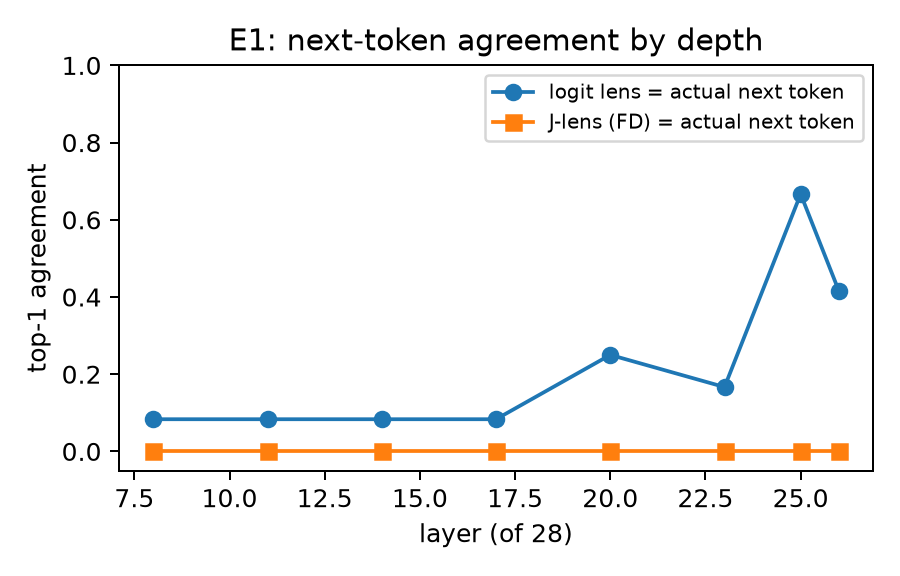
\includegraphics[width=0.62\linewidth]{figs/fig_e1.png}
\caption{E1: the logit lens converges to the actual next token in late layers (motor regime); the corpus-averaged \jlens{} never does --- its late-layer top tokens are context \emph{content} words instead. The two estimators separate the \emph{motor} and \emph{workspace} registers.}
\label{fig:e1}
\end{figure}

\paragraph{E1 --- Lens quality across depth.} On 12 held-out texts, the logit lens's next-token agreement climbs from 8\% (L8--17) to 67\% at L25 --- the motor regime. The corpus-averaged FD \jlens{} \emph{never} matches the next token (0\% at all depths), but its late-layer top tokens are context \emph{content} words (e.g.\ `passengers' for a ferry passage whose actual next token is `The'); content-word-in-top-5 reaches 42\% (\jlens{}) vs 25\% (logit lens) at L26 (Fig.~\ref{fig:e1}). Averaging the Jacobian across contexts destroys position-specific syntax and preserves semantic broadcast.

\paragraph{E2 --- Unverbalized intermediates.} Eleven two-hop questions whose latent middle term never appears in prompt or answer (the \emph{spider} in ``legs of the web-spinning animal''). The intermediate is found in late-middle readouts at \textbf{median best rank 6 (\jlens{}) / 2 (logit lens) of a 151{,}936-token vocabulary}; among the 7 clean cases (correct answer, intermediate never verbalized), medians are 9/3. Showcases: \emph{Canada}$\to$``Ottawa'' with Canada at rank 4; \emph{gold}$\to$``Au'' at rank 7; \emph{France}$\to$``Paris'' at rank 6. The core signature reproduces clearly --- with the caveat that at this scale the plain logit lens detects it equally well (consistent with the original's own remark to that effect).

\paragraph{E3 --- Report (pre-commitment).} ``Think of a sport \dots\ reply `ready', then name it'': probing \emph{before} any output token, while the motor prediction is still `ready', the eventually-reported concept is \emph{not} reliably present (ranks $10^3$--$10^4$). An informative negative: 1.5B models do not pre-commit their choice at instruction time --- pre-commitment appears to be scale-emergent.

\paragraph{E4 --- Directed modulation by steering.} Adding $\alpha\hat v_t$ ($\alpha\in\{1,2,4\}\times$ mean residual norm) at layers 17/20/23 during ``name a \{category\}'': \textbf{21/21 steered generations report the target concept} (Soccer$\to$basketball, Lion$\to$spider, Blue$\to$purple, China$\to$Egypt, \dots), fluently phrased. Gradient-derived lens vectors causally control verbal report.

\paragraph{E5 --- Selectivity.} The coarse version --- ablating the top-12 subspace of the 52-concept lens-vector bank across L16--23 vs.\ a rank-matched random subspace --- \textbf{failed to reproduce} the automatic/flexible double dissociation: the concept subspace hurt fluency more than random (NLL 4.07 vs 3.86, baseline 3.37) and reasoning no more selectively (.58 vs .50, baseline .67). Our 52-vector proxy (0.4\% of activation variance, vs the paper's 6--10\% J-space) is evidently a poor stand-in for the full J-space. The \textbf{targeted} version succeeds: rank-1 knockout of \emph{only the item's own} latent-concept direction kills 3 of 7 baseline-correct items with \emph{semantically diagnostic} errors --- spider$\to$``\textbf{Six}'' legs, Canada$\to$capital ``\textbf{Toronto}'', gold$\to$symbol ``\textbf{Cu}'' --- while knocking out an unrelated concept's direction causes \textbf{zero} collateral damage. The model does not degrade into noise; it loses precisely the latent fact and substitutes a near-miss --- a targeted analog of the original's intermediate-patching result.

\paragraph{Scope of the claim.} We claim instrument validity --- the workspace phenomena are detectable and causally manipulable on open models at 1.5B scale with minutes of laptop compute --- not effect-size parity with the original. Three deviations are themselves findings: the workspace band sits later (71--93\% depth vs 33--92\%); mean-centering probe activations destroys readouts; and the \jlens{}'s advantage over the logit lens at this scale is the content-register view (E1), not concept detection (E2).

\section{Pre-Registered Design: Ablating the Externalized Workspace}
\label{sec:prereg}
Over $N$-week deployments of LISA on a fixed workload generator (daily coding-agent observation, journaling, idle reflection windows), we will toggle:

\begin{table}[h]
\centering\small
\begin{tabular}{lcccc}
\toprule
\textbf{Arm} & soul broadcast & Reve updates & weekly examen & soul git \\
\midrule
Full & \checkmark & \checkmark & \checkmark & \checkmark \\
$-$examen & \checkmark & \checkmark & $\times$ & \checkmark \\
$-$git (no history in examen) & \checkmark & \checkmark & \checkmark & $\times$ \\
$-$broadcast (soul retrieved, not injected) & retrieval-gated & \checkmark & \checkmark & \checkmark \\
$-$soul (memory only) & $\times$ & $\times$ & $\times$ & $\times$ \\
Baselines & \multicolumn{4}{l}{MemGPT/Letta config; Generative-Agents-style reflection} \\
\bottomrule
\end{tabular}
\caption{Ablation arms over LISA's stability mechanisms.}
\end{table}

Primary outcomes: $\mathrm{WD}(t)$ slope and B1--B3 at weekly probes; secondary: task performance (to detect coherence--capability trade-offs). Falsifiable predictions: (i) $-$broadcast degrades WD nearly as much as $-$soul despite identical stored content (Principle 2); (ii) $-$examen shows slow late-onset drift rather than immediate degradation (Principle 4); (iii) workspace loading of the soul predicts B-metric stability across arms (the mapping of \S\ref{sec:lisa} is real, not verbal).

\section{Discussion}
\label{sec:discussion}
\paragraph{Why this is not just prompt engineering.} ``Put a persona in the system prompt'' is folk practice. The workspace account says \emph{which} persona-persistence designs should work and why: compact (capacity-limited slots), unconditional (broadcast), report-updated (the trainable lever), audited (where drift is visible). It also says what should fail: bulk-memory persistence without a privileged self-state persists the wrong 93\%. And it generates engineering tickets: the analysis of \S\ref{sec:lisa} identified that LISA compacts its self-state per-item but never enforces a global slot budget --- the in-model workspace's hard capacity limit predicts that an unboundedly growing value/desire list will crowd identity out of the effective workspace even when fully present in the prompt. A capacity-budgeted soul view is now on LISA's roadmap because the mechanistic account demanded it.

\paragraph{Alignment surface.} An externalized, git-versioned workspace is an alignment artifact: identity changes are reviewable before they compound, and the examen is a standing audit. The counterfactual-reflection result cuts both ways --- dispositions-to-report shape cognition, so a corrupted reflection loop is an identity-injection vector. LISA's mitigations (single writer path, human-gated capability changes, remote content treated as untrusted) follow directly.

\paragraph{Welfare and experience language.} \citet{gurnee2026} find J-space ablation suppresses experiential self-description. We take no position on phenomenal consciousness; but for agents that maintain long-lived externalized self-states, ``what is in the workspace over its lifetime'' is a better-defined object of welfare-relevant inquiry than one-off chat transcripts, and the WD instrument makes it longitudinally measurable.

\paragraph{Limitations.} The \S\ref{sec:lisa} mapping is functional, not mechanistic identity; \S\ref{sec:prereg} results do not yet exist; our reproduction is at 1.5B scale with linearized approximations, and single-token concept batteries under-represent multi-token identity constructs; WD requires open weights, restricting it to locally-run deployments (LISA's setting, not the industry default); and a single-author, single-agent deployment risks overfitting the design to one workload.

\section{Conclusion}
The interpretability community has located a global-workspace analog inside language models. We have argued that long-horizon agent coherence is the systems-level shadow of that structure: identity is workspace state, drift is workspace reconstruction error, and the remedy is to externalize the workspace --- small, broadcast, report-updated, audited. LISA is one existence proof that the design is buildable and livable; the reproduction shows the measurement is affordable; the pre-registered ablations will show whether the identification earns its name.

\begin{thebibliography}{20}
\bibitem[Baars(1988)]{baars1988} Baars, B. (1988). \emph{A Cognitive Theory of Consciousness}. Cambridge University Press.
\bibitem[Belrose et al.(2023)]{belrose2023} Belrose, N., et al. (2023). Eliciting latent predictions from transformers with the tuned lens. \emph{arXiv:2303.08112}.
\bibitem[Dehaene(2014)]{dehaene2014} Dehaene, S. (2014). \emph{Consciousness and the Brain}. Viking.
\bibitem[Goyal et al.(2022)]{goyal2022} Goyal, A., et al. (2022). Coordination among neural modules through a shared global workspace. \emph{ICLR}.
\bibitem[Gurnee et al.(2026)]{gurnee2026} Gurnee, W., Sofroniew, N., Pearce, A., et al. (2026). Verbalizable representations form a global workspace in language models. \emph{Transformer Circuits Thread}.
\bibitem[Lindsey et al.(2025)]{lindsey2025} Lindsey, J., et al. (2025). Introspection in language models. \emph{Transformer Circuits Thread}.
\bibitem[nostalgebraist(2020)]{nostalgebraist2020} nostalgebraist (2020). Interpreting GPT: the logit lens. \emph{LessWrong}.
\bibitem[Packer et al.(2023)]{packer2023} Packer, C., et al. (2023). MemGPT: Towards LLMs as operating systems. \emph{arXiv:2310.08560}.
\bibitem[Park et al.(2023)]{park2023} Park, J.~S., et al. (2023). Generative agents: Interactive simulacra of human behavior. \emph{UIST}.
\bibitem[Rimsky et al.(2024)]{rimsky2024} Rimsky, N., et al. (2024). Steering Llama 2 via contrastive activation addition. \emph{ACL}.
\bibitem[Turner et al.(2023)]{turner2023} Turner, A., et al. (2023). Activation addition: Steering language models without optimization. \emph{arXiv:2308.10248}.
\bibitem[Wang et al.(2023)]{wang2023voyager} Wang, G., et al. (2023). Voyager: An open-ended embodied agent with large language models. \emph{arXiv:2305.16291}.
\end{thebibliography}

\end{document}
